\documentclass[12pt]{article}

\usepackage[utf8]{inputenc}
\usepackage[a4paper, total={6in, 10in}]{geometry}
\usepackage{tikz}
\usepackage{forest}

\tikzset{state/.style={draw,circle}}
\forestset{d/.style={dotted,edge=dotted},
r/.style={red,edge=red}}

\usetikzlibrary{arrows, automata}
\usetikzlibrary{positioning}

%--------------------------------------------------
% Node definitions for figure
%--------------------------------------------------
% Black node 
\tikzstyle{black_node} = [
    circle, 
    white, 
    font=\bfseries, 
    draw=black, 
    fill=black, 
    align=center, 
    inner sep=2pt, % 2pt is good for two digits
    text width=1.5em, 
    text centered
]

% Red node
\tikzstyle{red_node} = [
    circle, 
    white, 
    font=\bfseries, 
    draw=black,
    fill=red,
    align=center, 
    inner sep=2pt, % 2pt is good for two digits
    text width=1.5em, 
    text centered
]

% NIL node - drawn as black rounded rectangles
\tikzstyle{nil} = [
    rounded corners, 
    white,
    draw=black, 
    fill=black,
    align=center, 
    inner sep=0pt, 
    minimum width=1.0em, 
    minimum height=1.0em
]

\begin{document}

%--------------------------------------------------
% Sample red-black trees
%--------------------------------------------------
% Example 1
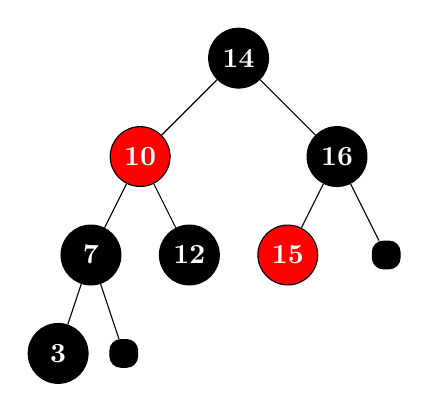
\begin{tikzpicture}[
    %-,
    %>=stealth', 
    level/.style={
        sibling distance = 2.5cm/#1, 
        level distance = 1.25cm
    }
] 
\node [black_node] {14}
    child{ node [red_node] {10}
        child{ node [black_node] {7} 
            child{ node [black_node] {3} }
            child{ node [nil] {} }
        }
        child{ node [black_node] {12} }
    }
    child{ node [black_node] {16}
        child{ node [red_node] {15} }
        child{ node [nil] {} }
    }
; 

%\draw [<-, ultra thick] (leaf 5) -- node [auto] {$y$} ++(135:1cm) ;
\end{tikzpicture}

\newpage

% Example 2: supplementary explanation for case 1
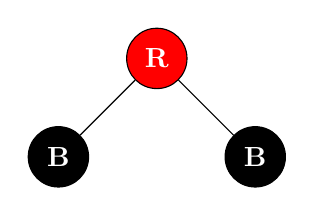
\begin{tikzpicture}[
    level/.style={
        sibling distance = 2.5cm/#1, 
        level distance = 1.25cm
    }
] 
\node [red_node] {R}
    child{ node [black_node] {B} }
    child{ node [black_node] {B} }
; 
\end{tikzpicture}

% Example 3: supplementary explanation for case 2-3
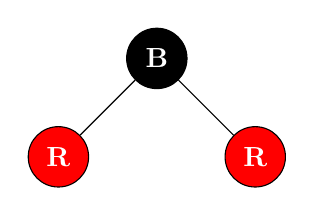
\begin{tikzpicture}[
    level/.style={
        sibling distance = 2.5cm/#1, 
        level distance = 1.25cm
    }
] 
\node [black_node] {B}
    child{ node [red_node] {R} }
    child{ node [red_node] {R} }
; 
\end{tikzpicture}

\newpage

%--------------------------------------------------
% Figures for my explanation on red-black tree insertion
%--------------------------------------------------
\begin{forest}
for tree={state,edge={-},grow=south,l sep=6mm,s sep=10mm},
[22,d
 [13,d
  [30,red,edge=dotted
   [15,r]
   [85,r]{\draw[<->,red] () to[bend right=45] node[midway,above
   right,font=\small]{zam} (!u.east);}
  ]
  [71
   [17]
   [20]
  ]
 ]
 [11,d
  [33,edge=dotted
   [32]
  ]
  [55,d]
 ]
]
\end{forest}

\end{document}
